
\documentclass{article}
\usepackage[utf8]{inputenc}
\usepackage[spanish]{babel}
\usepackage{graphicx}
\usepackage{geometry}
\usepackage{enumerate}
\usepackage{titlesec}
\usepackage{float}

\geometry{letterpaper, margin = 1.5cm}

%Datos de la Portada
\title{Introduccion a la Programacion \\ Practica 3}
\author{Medina Martinez Jonathan Jason \\ 2023640061}
\date{13 de marzo de 2023}

\begin{document} %Inicio del Documento

\fontsize{12}{16}\selectfont

\begin{figure}[t] %Logos Portada


\includegraphics[width=2.5 cm]{Logo1.jpeg}
\hfill

\includegraphics[width=3 cm]{Logo2.png}

\end{figure}

\maketitle %Titulo Portada
\newpage

\tableofcontents %Indice
\newpage

\section{Objetivo}

Desarrollo de programas utilizando las sentencias de control.

\
\
\

\section{Introducción}

En esta practica se realizaran diversos programas en c utilizando diversos, principalmente sentencias de control como \textbf{switch-case}, \textbf{do-while}, \textbf{while} y \textbf{for}.

\newpage

\section{Desarrollo}
\subsection{Programa 1}

Programa que calcule el area y el perımetro de diversas figuaras que permita al usuario escoger atravez de un menu.

\

\begin{figure}[H]
    \centering
    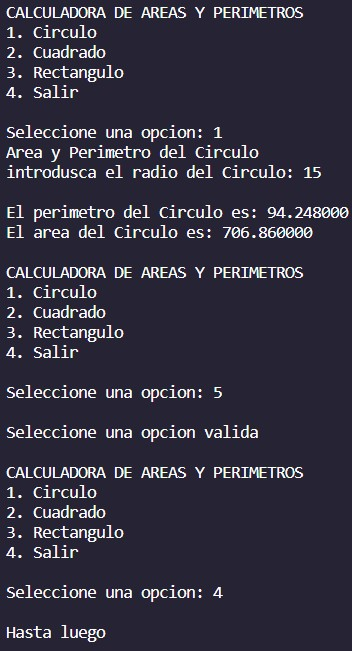
\includegraphics[width = 10cm]{img1.jpg}
\end{figure}
\newpage
\subsection{Programa 2}

Programa que solicite al usuario un numero e imprima el triangulo de Floyd de tal forma que los pares sean representados con 1 y los impares con 0.

\

\begin{figure}[H]
    \centering
    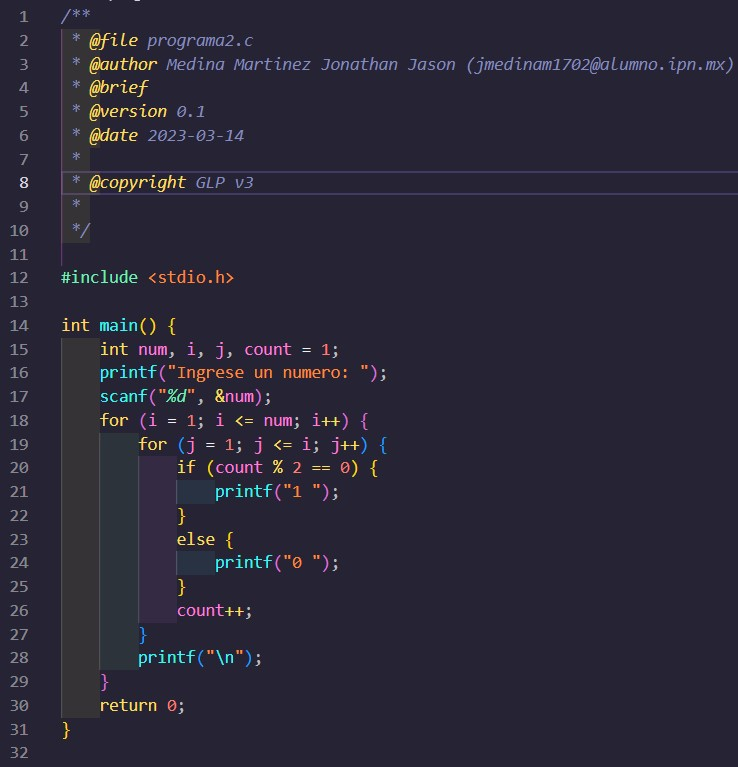
\includegraphics[width = 15cm]{img2a.jpg}
\end{figure}
\begin{figure}[H]
    \centering
    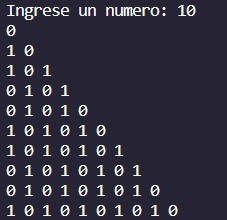
\includegraphics[width = 10cm]{img2b.jpg}
\end{figure}
\newpage
\subsection{Programa 3}

Programa que solicite al usuario un numero n e imprima en pantalla la sucesion de Fibonacci hasta el termino n, utilizando un ciclo for.

\

\begin{figure}[H]
    \centering
    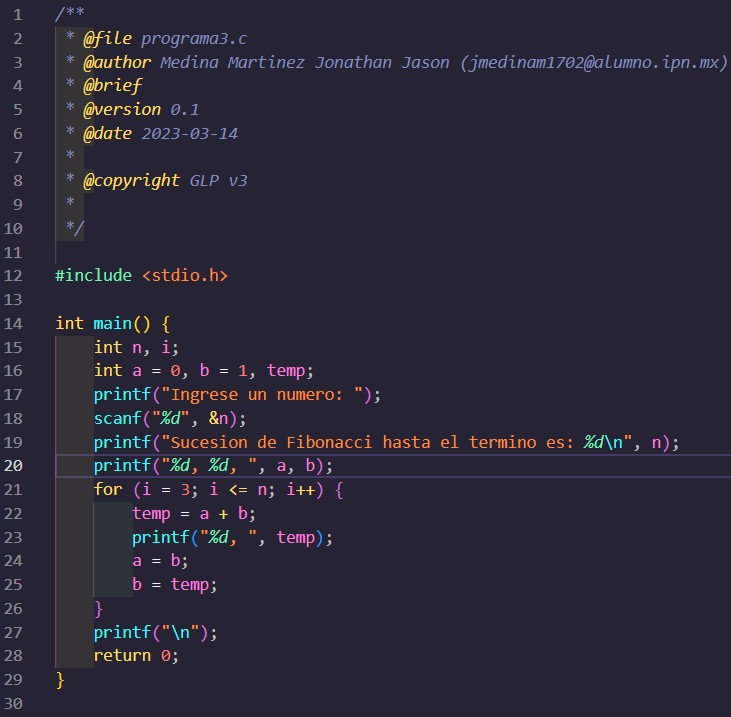
\includegraphics[width = 15cm]{img3a.jpg}
\end{figure}
\begin{figure}[H]
    \centering
    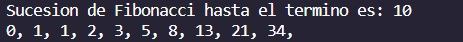
\includegraphics[width = 10cm]{img3b.jpg}
\end{figure}
\newpage
\subsection{Programa 4}

Repita el programa anterior pero utilizando un ciclo while.

\

\begin{figure}[H]
    \centering
    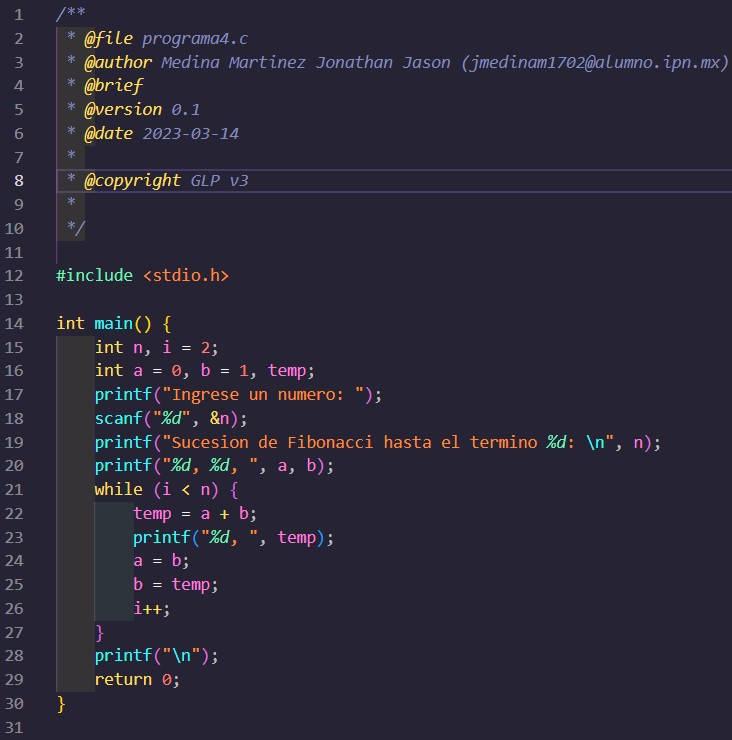
\includegraphics[width = 15cm]{img4a.jpg}
\end{figure}
\begin{figure}[H]
    \centering
    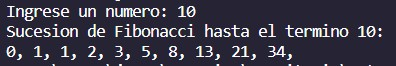
\includegraphics[width = 10cm]{img4b.jpg}
\end{figure}
\newpage
\subsection{Programa 5}

Programa que solicite al usuario un numero e imprima en pantalla su factorial, utilizando un ciclo for.

\begin{figure}[H]
    \centering
    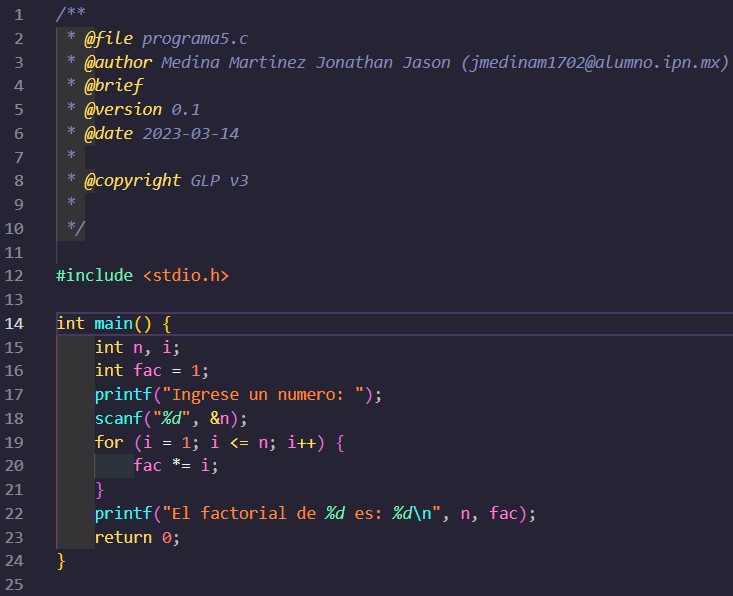
\includegraphics[width = 15cm]{img5a.jpg}
\end{figure}
\begin{figure}[H]
    \centering
    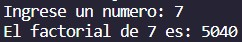
\includegraphics[width = 10cm]{img5b.jpg}
\end{figure}
\newpage
\subsection{Programa 6}

Repita el programa anterior pero utilizando un ciclo while.

\begin{figure}[H]
    \centering
    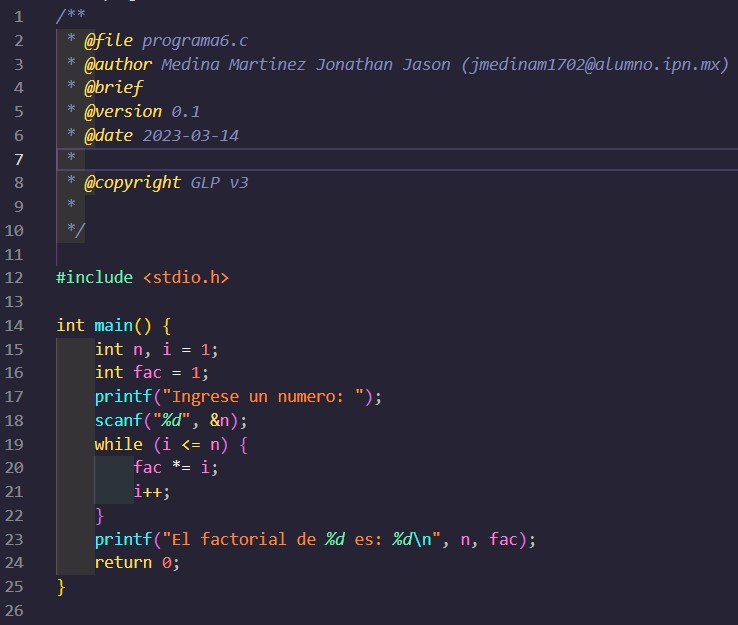
\includegraphics[width = 15cm]{img6a.jpg}
\end{figure}
\begin{figure}[H]
    \centering
    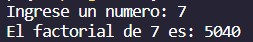
\includegraphics[width = 10cm]{img6b.jpg}
\end{figure}
\newpage
\subsection{Programa 7}

Programa que solicite al usuario un numero n e imprima n terminos de la serie
armonica y su suma hasta tres decimales, utilizando un ciclo for.

\begin{figure}[H]
    \centering
    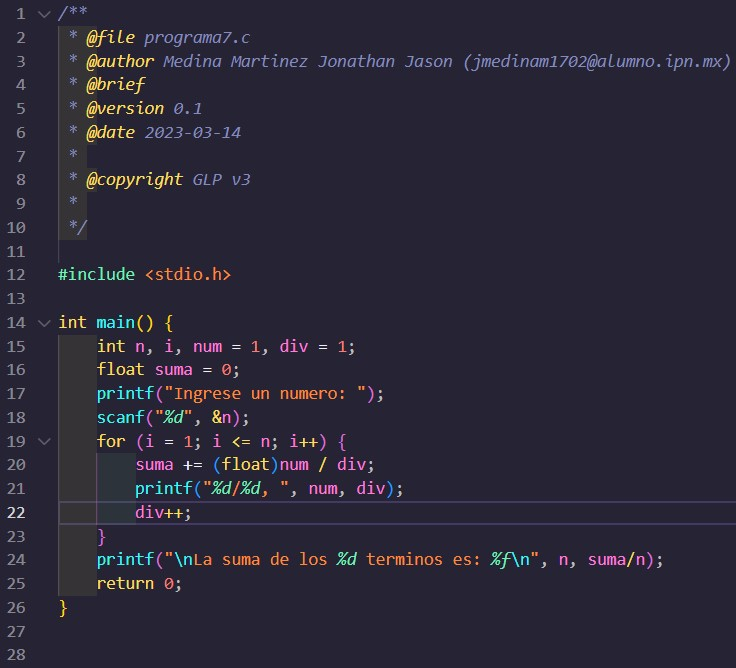
\includegraphics[width = 15cm]{img7a.jpg}
\end{figure}
\begin{figure}[H]
    \centering
    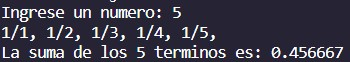
\includegraphics[width = 10cm]{img7b.jpg}
\end{figure}
\newpage
\subsection{Programa 8}

Repita el programa anterior pero utilizando un ciclo while.

\begin{figure}[H]
    \centering
    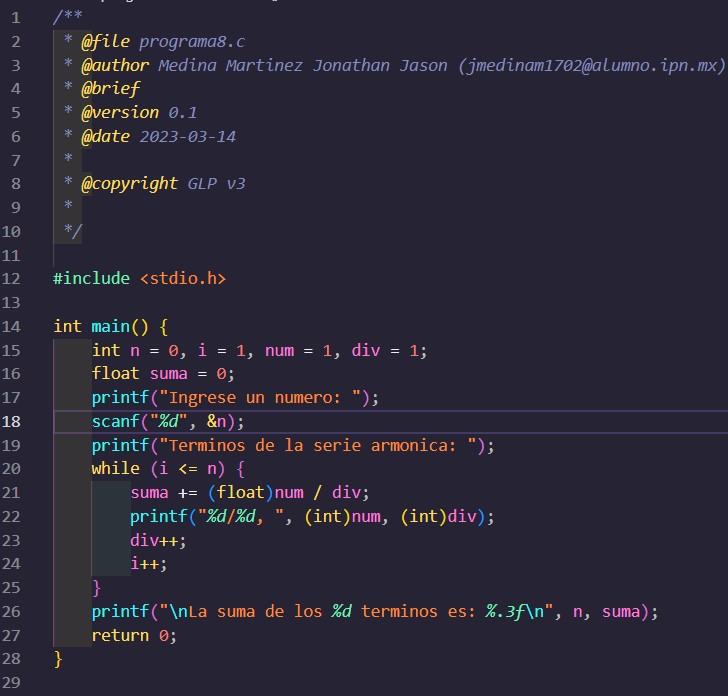
\includegraphics[width = 15cm]{img8a.jpg}
\end{figure}
\begin{figure}[H]
    \centering
    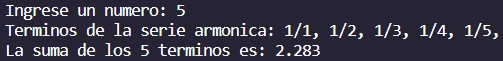
\includegraphics[width = 10cm]{img8b.jpg}
\end{figure}
\newpage
\subsection{Programa 9}

Programa que solicite al usuario un numero e imprima el triangulo de Floyd de tal forma que los pares sean representados con 1 y los impares con 0.

\begin{figure}[H]
    \centering
    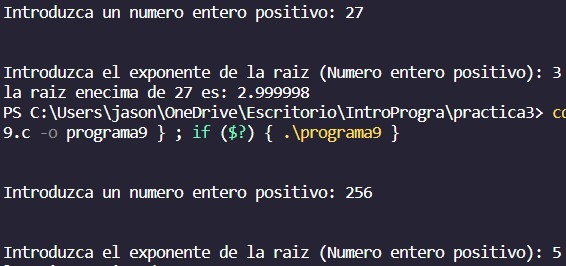
\includegraphics[width = 15cm]{img9a.jpg}
\end{figure}
\begin{figure}[H]
    \centering
    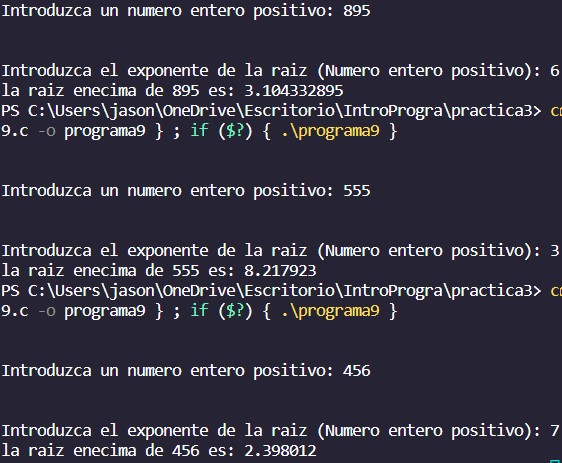
\includegraphics[width = 10cm]{img9b.jpg}
\end{figure}
\newpage
\subsection{Programa 10}

Repita el programa anterior pero utilizando un ciclo while.

\begin{figure}[H]
    \centering
    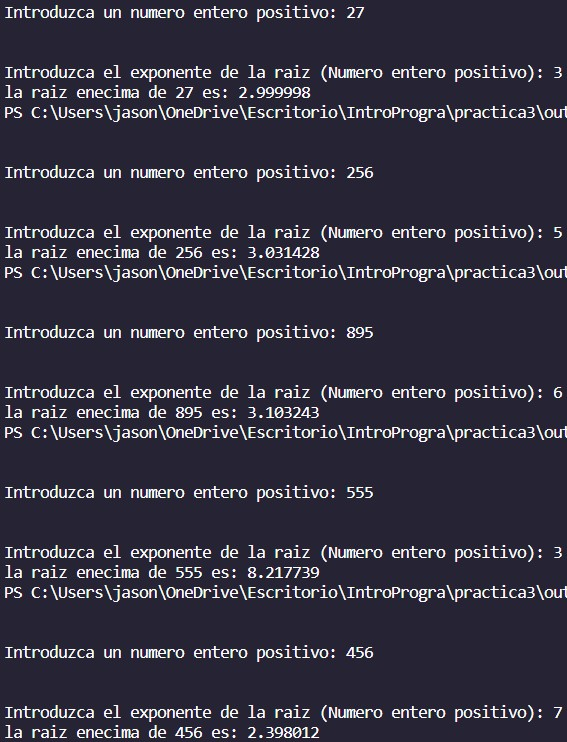
\includegraphics[width = 10cm]{img10.jpg}
\end{figure}

\
\
\
\

\section{Conclusion}

En esta practica realizamos distintos tipos de programas que nos permiten obtener resultados por medio de sentencias de control para realizar ciclos.

\end{document}